%\newsection{Kapitel1}

%Hier den Inhalt mit \input einfügen und die folgenden Zeilen entfernen


%%%%%%%%%%%%%%%%%%%%%%%%%%%%%%%%%%%%%%%%%%%%%%%%% Anfang - Induktivität %%%%%%%%%%%%%%%%%%%%%%%%%%%%%%%%%%%%%%%%%%%%%%

	\section{Induktivität und Spule}

	\s{
	Das Gegenstück zum Kondensator ist die Spule, oder genauer gesagt: Das Gegenstück zur Kapazität $C$ ist die Induktivität $L$.
	Die Induktivität ist ebenfalls ein Energiespeicher, wobei der Unterschied in der Art der genutzten Felder liegt.
	Während bei der Kapazität die Energie in Form eines elektrischen Feldes gespeichert wird,
	geschieht dies bei der Induktivität über das magnetische Feld.
	}
%%%%%%%%%%%%%%%%%%%%%%%%%%%%%%%%%%%%%%%%%%%%%%%%% Anfang - Lernziele Induktivität %%%%%%%%%%%%%%%%%%%%%%%%%%%%%%%%%%%%%%%%%%%%%%
\begin{frame}
	\ftx{Lernziele: Induktivität und Spule}
\begin{Lernziele}{Induktivität und Spule}
		Die Studierenden
		\begin{itemize}
		\item können zwischen Induktivität und Spule differenzieren.
		\item kennen die wichtigsten Parameter rund um die Induktivität und die Spule.
		\item können die Induktivität einer Spule berechnen.
	\end{itemize}
	\end{Lernziele}
\end{frame}
%%%%%%%%%%%%%%%%%%%%%%%%%%%%%%%%%%%%%%%%%%%%%%%%% Ende - Lernziele Induktivität %%%%%%%%%%%%%%%%%%%%%%%%%%%%%%%%%%%%%%%%%%%%%%

	\subsection{Die Induktivität $L$} \label{sec:Induktivität}
\s{
	Die Induktivität ist die Fähigkeit eines Objektes, elektrische Energie in Form eines magnetischen Feldes zu speichern.
	Diese Eigenschaft kommt zustande, sobald ein elektrischer Strom durch einen Leiter fließt um welchen sich entsprechend ein magnetisches Feld ausbildet.
	Das Formelzeichen der Induktivität ist $L$ (benannt nach dem französischen Physiker Heinrich Lenz), während die Einheit in Henry ($\mathrm{H}$) angegeben wird.

	Das einfachste und geläufigste Beispiel, an dem die Induktivität erklärt werden kann, ist die Spule.
	Obwohl sich das Phänomen der Induktivität bereits bei einem einfachen Leiter ausbildet, wird dieser Effekt durch den Aufbau einer Spule bewusst verstärkt.
	In Abbildung \ref{fig:Spule} ist ein Zylinderluftspule mit ihrer magnetischen Flussdichte $\vec{B}$ dargestellt.
}
%%%%%%%%%%%%%%%%%%%%%%%%%%%%%%%%%%%%%%%%%%%%%%%%% Anfang - Grafik Spule ohne Kern %%%%%%%%%%%%%%%%%%%%%%%%%%%%%%%%%%%%%%%%%%%%%%
% Spule ohne Kern
\begin{frame}
	\ftx{Magnetisches Feld einer Zylinderluftspule}
	\begin{figure}[H]
		\centering
			\includesvg[width=0.6\textwidth]{Magnetisches_Feld_Spule}
			\s{\caption{\textbf{Darstellung des magnetischen Feldes einer Zylinderluftspule.} Es illustriert die Feldlinien sowohl innerhalb als auch außerhalb der Spule
			und veranschaulicht, wie sich das Magnetfeld entlang  der Achse der Spule konzentriert und außerhalb der Spule abnimmt.}}
			\label{fig:Spule}
		\end{figure}
\end{frame}
%%%%%%%%%%%%%%%%%%%%%%%%%%%%%%%%%%%%%%%%%%%%%%%%% Ende - Grafik Spule ohne Kern %%%%%%%%%%%%%%%%%%%%%%%%%%%%%%%%%%%%%%%%%%%%%%
\s{
Das Thema der magnetischen Größen wird ausführlich in Modul 6 behandelt.
Zum Verständnis der Funktionsweise einer Spule und der daraus resultierenden Induktivität,
soll eine kurze Einführung zur Entstehung von Magnetismus helfen.

Sobald Strom durch einen geraden Leiter fließt, entsteht ein magnetisches Feld konzentrisch um den Leiter herum.
Abhängig von Stromstärke und Stromrichtung ändert sich auch das magnetische Feld.
Die Rechte-Faust-Regel dient dabei als Gedankenstütze zur Bestimmung der Richtung und Orientierung des Magnetfeldes.
}
%%%%%%%%%%%%%%%%%%%%%%%%%%%%%%%%%%%%%%%%%%%%%%%%% Anfang - Grafik Lenzsche Regel %%%%%%%%%%%%%%%%%%%%%%%%%%%%%%%%%%%%%%%%%%%%%%
\begin{frame}
	\ftx{Die Rechte-Hand-Regel}
	\begin{figure}[H]
		\centering
			\includesvg[width=1\textwidth]{Rechte-Faust-Regel}
			\s{\caption{\textbf{Rechte-Hand-Regel zur Bestimmung der Richtung des Magnetfeldes.} Ein stromdurchflossenen Leiter erzeugt ein Magnetfeld das mit
			hilfe der Rechten-Hand-Regel bestimmt wird. Wenn der Daumen der rechten Hand in die Richtung des Stroms zeigt, dann krümmen sich die übrigen Finger in
			die Richtung der Feldlinien des Magnetfeldes.}}
			\label{fig:Rechtehand}
		\end{figure}
\end{frame}
%%%%%%%%%%%%%%%%%%%%%%%%%%%%%%%%%%%%%%%%%%%%%%%%% Ende - Grafik Lenzsche Regel %%%%%%%%%%%%%%%%%%%%%%%%%%%%%%%%%%%%%%%%%%%%%%


\s{
Entsprechend der Grafik \ref{fig:Rechtehand} verläuft das Magnetfeld in Richtung der Fingerspitzen konzentrisch um den Leiter herum, sofern man den Daumen in Richtung der technischen Stromrichtung,
also entgegen der Fließrichtung der Elektronen, ausrichtet. Das Magnetfeld dreht sich von Süd nach Nord und hat eine Flussdichte $\vec{B}$, sowie eine Feldstärke $\vec{H}$.
Dabei ist zu beachten, dass sich die magnetische Flussdichte $\vec{B}$ analog zur elektrischen Feldstärke $\vec{E}$ , und die magnetische Feldstärke $\vec{H}$ analog zur elektrischen Flussdiche $\vec{D}$, verhält.
Im Modul 6 wird das Thema Magnetismus ausführlicher behandelt. In diesem Modul geht es primär um das Kennenlernen der Spule und der Induktivität.
}

%%%%%%%%%%%%%%%%%%%%%%%%%%%%%%%%%%%
\begin{frame}
	\ftx{Induzierte Spannung}
	\b{
		\begin{equation*}
			U_\mathrm{i} \sim \frac{\mathrm{d}\phi}{\mathrm{d}t}
		\end{equation*}

		\begin{equation*}
			U_\mathrm{i}= -N \cdot \frac{\mathrm{d}\phi}{\mathrm{d}t}
		\end{equation*}

		\begin{equation*}
			U_\mathrm{i} \sim \frac{\mathrm{d}I}{\mathrm{d}t}
		\end{equation*}

		\begin{equation*}
			U_\mathrm{i}= -L \cdot \frac{\mathrm{d}I}{\mathrm{d}t}
		\end{equation*}
	}
\end{frame}
\s{
	Der britische Physiker und Chemiker Michael Faraday führte mitte des 19. Jahrhunderts Experimente durch,
	bei denen er eine Spule in der Nähe eines Magneten bewegte oder den Strom in einer benachbarten Spule veränderte.
	Dabei stellte er fest, dass sich die Größe der induzierten Spannung proportional zur Änderungsrate des Magnetfeldes verhält.

	\begin{equation}
		U_\mathrm{i} \sim \frac{\mathrm{d}\phi}{\mathrm{d}t}
	\end{equation}

	Faraday stellte fest, dass der Proportionalitätsfaktor von der Anzahl der Wicklungen der Spule abhängt.

	\begin{equation}
		U_\mathrm{i}= -N \cdot \frac{\mathrm{d}\phi}{\mathrm{d}t}
	\end{equation}

	Etwa zur gleichen Zeit entdeckte der amerikanische Physiker Joseph Henry das Phänomen der Selbstinduktion,
	wobei ein elektrischer Strom in einer Spule eine Spannung in der Spule selbst induzieren kann, wenn der Strom verändert wird.
	Auch hier wurde ein proportionales Verhalten festgestellt.

	\begin{equation}
		U_\mathrm{i} \sim \frac{\mathrm{d}I}{\mathrm{d}t}
	\end{equation}

	Diese Eigenschaft der Spule die durch das Speichern magnetischer Energie entsteht ist die Induktivität $L$,
	deren Einheit dem Physiker zu Ehren als Henry $[\mathrm{H}]$ benannt wurde.

	\begin{equation}
		U_\mathrm{i}= -L \cdot \frac{\mathrm{d}I}{\mathrm{d}t}
	\end{equation}

	Das Minus-Zeichen kommt daher, dass der induzierte Strom nach der Lenz'schen Regel seiner Ursache entgegenwirkt.
}% nur im Skript


%%%%%%%%%%%%%%%%%%%%%%%%%%%%%%%%%%%%%%%%%%%%%%%%% Anfang - Formeln Zeitabhängigkeit Induktivität	 %%%%%%%%%%%%%%%%%%%%%%%%%%%%%%%%%%%%%%%%%%%%%%
%%%%% Zeitabhängige Formeln für induktivität

\begin{frame}
\ftx{Zeitabhängige Formeln der Induktivität}
\b{
	$\bullet \quad $ Spannung über der Induktivität
	\begin{equation*}
		u_\mathrm{L}(t) = L \cdot \frac{di_\mathrm{L}(t)}{dt}
	\end{equation*}
	$\bullet \quad $ Strom durch die Induktivität
	\begin{equation*}
		i_\mathrm{L}(t) = \frac{1}{L} \cdot \int u_\mathrm{L}(t) \, dt
	\end{equation*}
}
\end{frame}

	\s{
		Analog zum Kondensator, kann auch das zeitabhängige Verhalten für die Spule folgendermaßen ausgedrückt werden:


	Spannung über der Induktivität
	\begin{equation}
		u_\mathrm{L}(t) = L \cdot \frac{di_\mathrm{L}(t)}{dt}
	\end{equation}
	Strom durch die Induktivität
	\begin{equation}
		i_\mathrm{L}(t) = \frac{1}{L} \cdot \int u_\mathrm{L}(t) \, dt
	\end{equation}
}

	%%%%%%%%%%%%%%%%%%%%%%%%%%%%%%%%%%%%%%%%%%%%%%%%% Ende - Formeln Zeitabhängigkeit Induktivität	 %%%%%%%%%%%%%%%%%%%%%%%%%%%%%%%%%%%%%%%%%%%%%%


%%%%%%%%%%%%%%%%%%%%%%%%%%%%%%%%%%%%


\subsection{Die Spule als Bauelement}

\s{
Mit dem Wissen über das magnetische Feld kann nun der Aufbau und die Funktionsweise der Spule erklärt werden. Ein einfaches Beispiel dafür ist die Zylinderluftspule.
Wird ein Leiter zu einer Leiterschleife geformt, bildet sich das Magnetfeld so aus, dass es durch die Schleifenöffnung hindurchgeht.
Werden nun mehrere Leiterschleifen hintereinander gewickelt, wird das Magnetfeld um den Faktor der Windungszahl verstärkt.
Diese Anordnung von gewickelten Leiterschleifen ergibt die in Abbildung \ref{fig:Luftspule} gezeigte Zylinderluftspule.
}

\begin{frame}
	\ftx{Die Spule als Bauelteil}
	\begin{figure}[H]
		\centering
			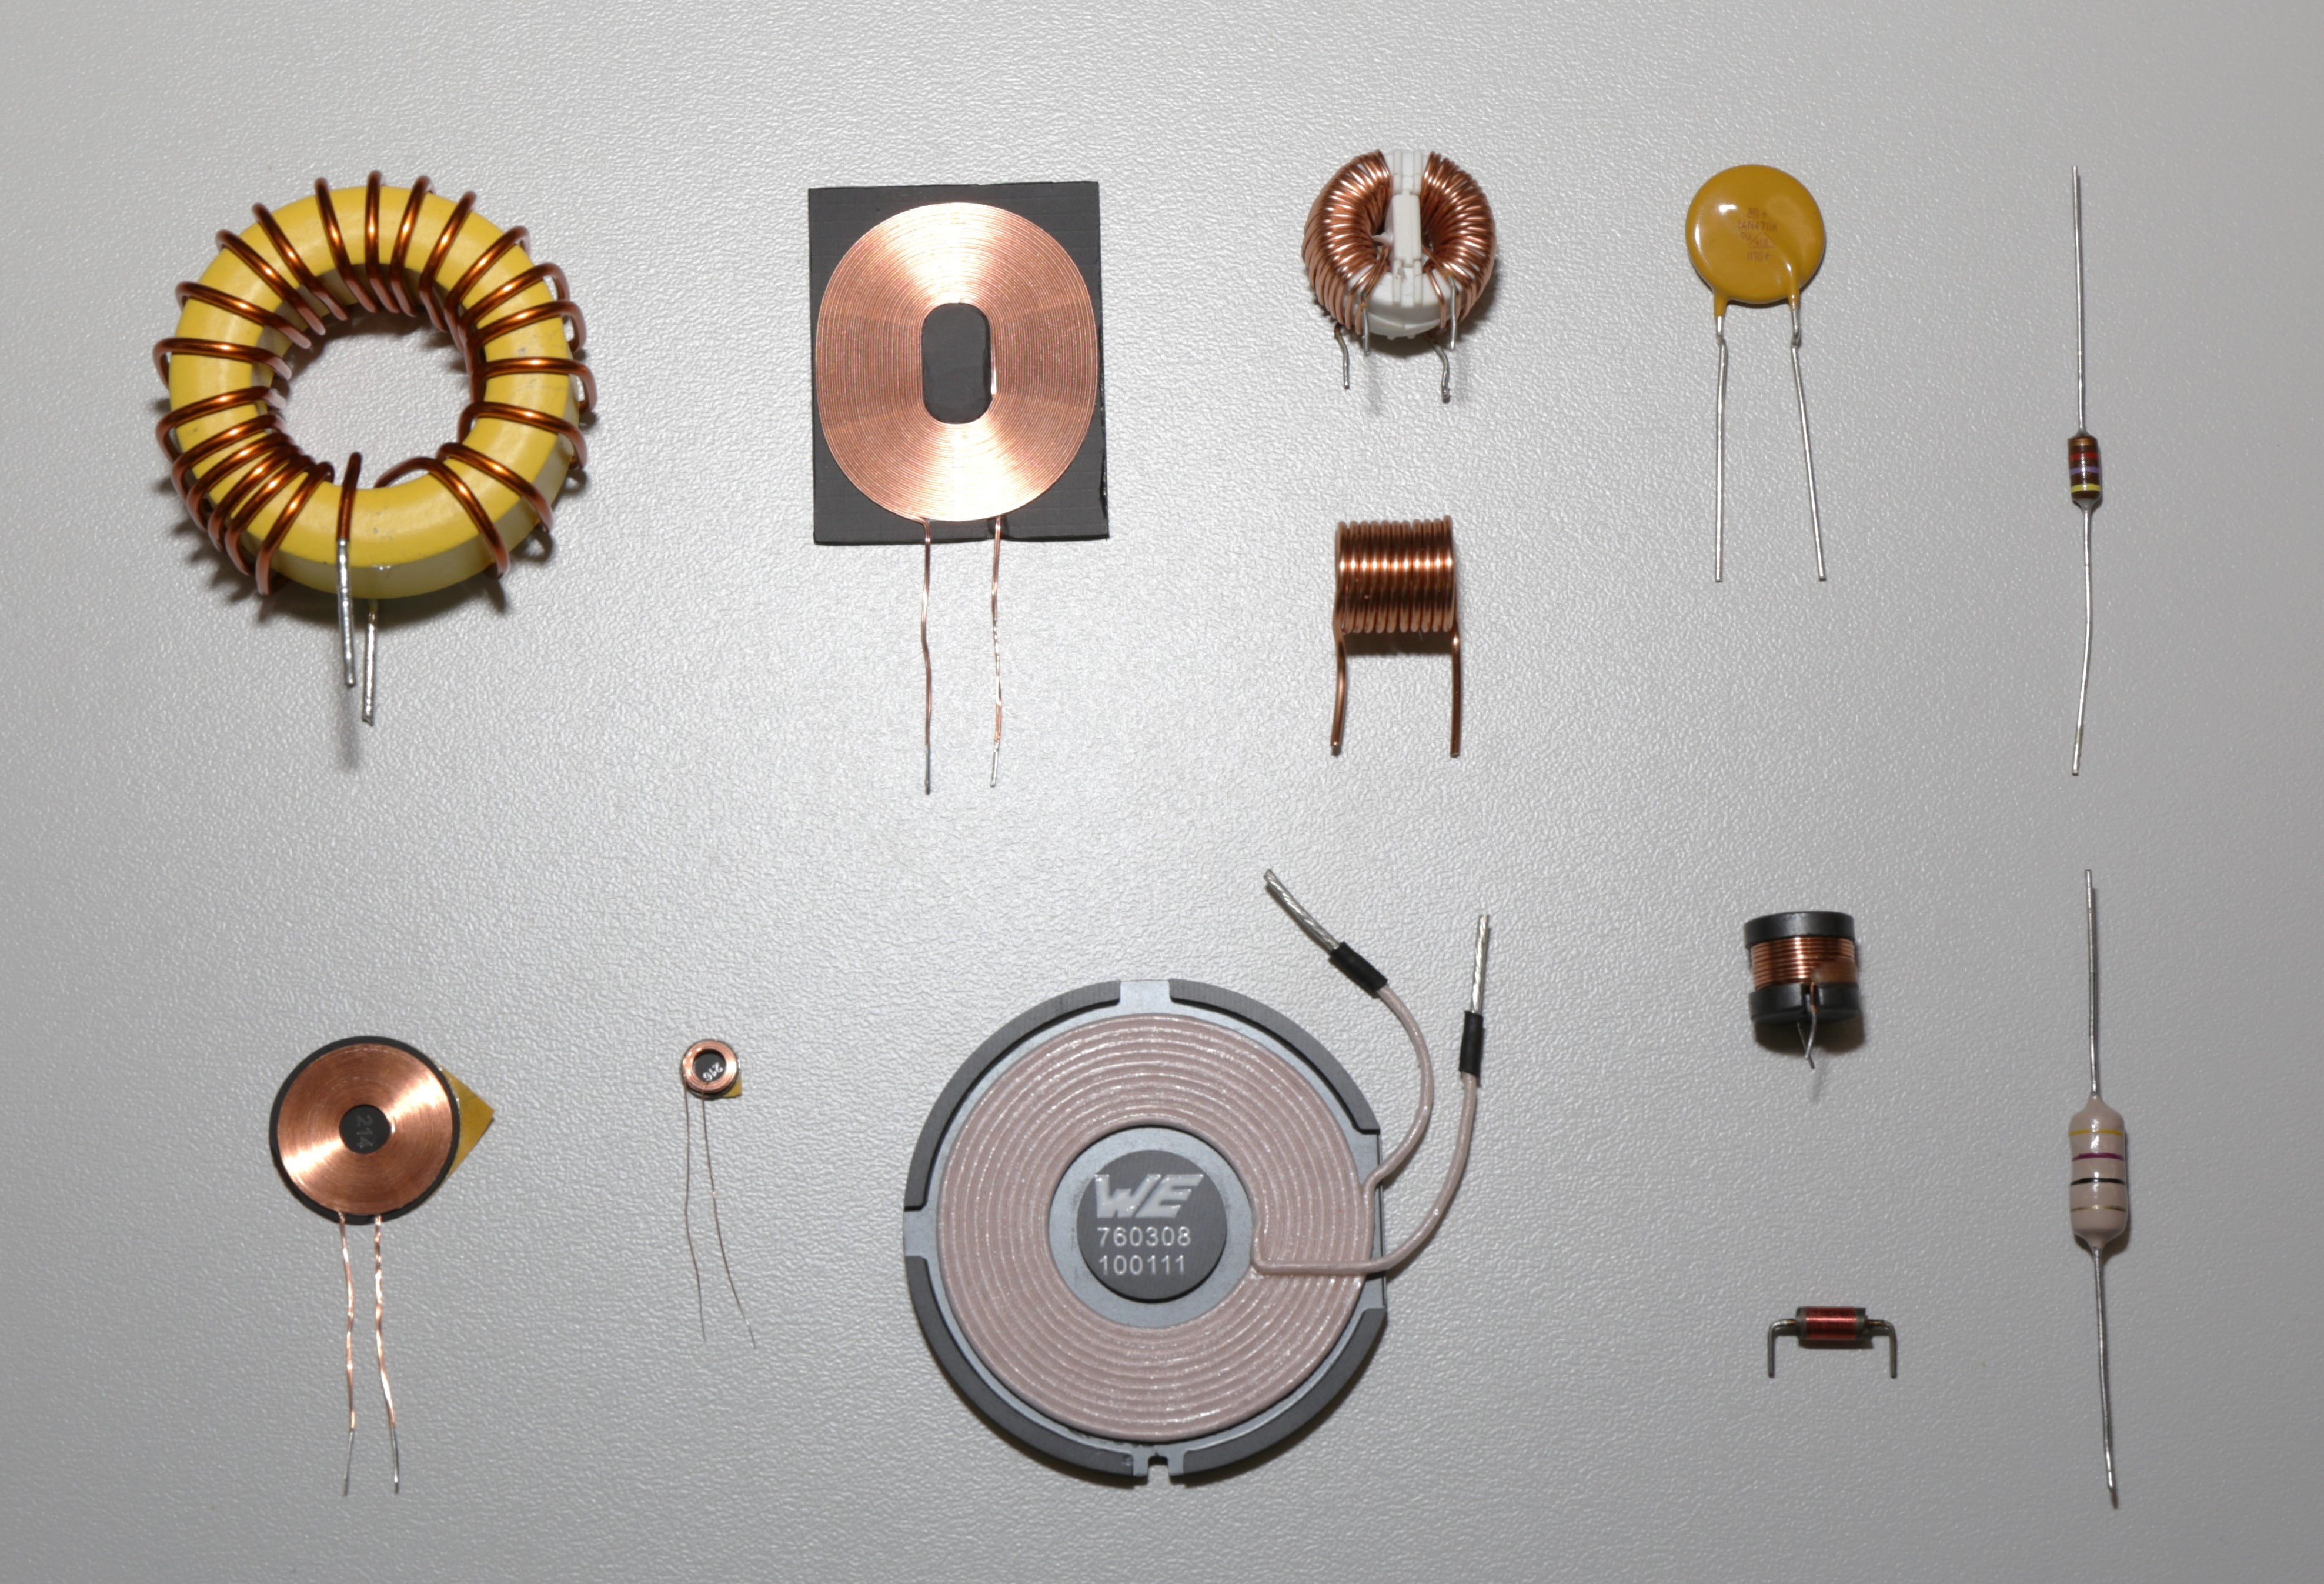
\includegraphics[width=0.7\textwidth]{sp}
			\s{\caption{\textbf{Verschiedene Arten und Bauformen von Spulen.} Darunter Zylinderspulen, Ringkernspulen, Eisenkernspulen und Luftspulen. Eine größere Anzahl von Windungen erhöht die Konzentration des Magnetfelds und steigert die Induktivität der Spule.
			 Ein Eisenkern kann zusätzlich verwendet werden, um die Magnetfeldlinien zu bündeln und die Effizienz zu verbessern.}}
			\label{fig:Luftspule}
		\end{figure}
\end{frame}
\s{
	Ihren Namen verdankt diese Spule ihrer zylindrischen Form in Längsrichtung und des Mediums Luft im inneren ihrer Wicklungen.
	Wenn nun ein Strom durch die Spule fließt, überlagern sich die Magnetfelder der einzelnen Wicklungen zu einem stärkeren Magnetfeld. Die Stärke hängt dabei von der Windungszahl
	und der Stromstärke, sowie der Entfernung zum Leiter, ab. Je nach Orientierung des Stromes und der Wicklungen, entsteht bei einer Zylinderluftspule auf der einen Seite ein
	Nord- und auf der anderen Seite ein Südpol. Der Verlauf der Magnetfeldlinien in einer Zylinderluftspule entspricht der Abbildung \ref{fig:Spule}. \\

	Was alle Spulen verbindet, ist ihre Fähigkeit, die Eigenschaft der Induktivität nutzbar zu machen,
	wie es im folgenden Schaltbild \ref{fig:Induktivität_ui} dargestellt ist. Dieses Schaltbild repräsentiert jedoch nur
	die idealisierte, nutzbare Induktivität.

	}% nur im Skript


%%%%%%%%%%%%%%%%%%%%%%%%%%%%%%%%%%%%%%%%%% Anfang - Schaltzeichen Induktivität EU, US	 %%%%%%%%%%%%%%%%%%%%%%%%%%%%%%%%%%%%%%%%%%%%%%
% Europäisches und amerikanisches Symbol
	\begin{frame}
		\ftx{Die Induktivität als Schaltugselement}
	\s{
		\begin{figure}[H]
		\centering
		\begin{circuitikz}
    % Europäisches Symbol
    \draw (0,0) to [L,i,v, name=L, o-, l=$L$] (2.5,0)
    to [short,-o] (2.5,0);

    % Amerikanisches Symbol
    \draw (6,0) to [L,i,v, name=L, o-, l=$L$, american] (8.5,0)
    to [short,-o] (8.5,0);

\end{circuitikz}
		\caption{\textbf{Schaltungselement für Spule.} Europäischen (links) und amerikanisches (rechts).}
		\label{fig:Induktivität_L_EU}
	\end{figure}
	}
%%%%%%%%%%%%%%%%%%%%%%%%%%%%%%%%%%%%%%%%%%%%%%%%% Ende - Schaltzeichen Induktivität	EU, US %%%%%%%%%%%%%%%%%%%%%%%%%%%%%%%%%%%%%%%%%%%%%%
%%%%%%%%%%%%%%%%%%%%%%%%%%%%%%%%%%%%%%%%%%%%%%%%% Anfang - Schaltzeichen Induktivität U,I	 %%%%%%%%%%%%%%%%%%%%%%%%%%%%%%%%%%%%%%%%%%%%%%
% Ideale Spule

	\begin{figure}[h]
		\begin{center}
		\begin{circuitikz}
    \draw (0,0)   to [L,i,v, name=L,o-, l={$L$}] (3,0)
    to [short,-o] (3,0);
    \varrmore{L}{$u_\mathrm{L}(t)$};
    \iarrmore{L}{$i_\mathrm{L}(t)$};

\end{circuitikz}
		\s{\caption{\textbf{Schaltzeichen einer idealen Spule.}}}
		\label{fig:Induktivität_ui}
		\end{center}
		\end{figure}
	\end{frame}
%%%%%%%%%%%%%%%%%%%%%%%%%%%%%%%%%%%%%%%%%%%%%%%%% Ende - Schaltzeichen Induktivität	U,I  %%%%%%%%%%%%%%%%%%%%%%%%%%%%%%%%%%%%%%%%%%%%%%%%%%%%%

\s{
	Für eine realitätsgetreue Nachbildung der Schaltung ist es wichtig die Spule als Bauteil
	vollständig zu beschreiben. Dies wird mit Hilfe eines Ersatzschaltbildes gemacht, welches auch die
	ungewollten, also parasitären Eigenschaften des Bauteils, nachbildet. Abbildung \ref{fig:Schaltbild einer realen Spule} zeigt ein solches
	Ersatzschaltbild.
}% nur im Skript
%%%%%%%%%%%%%%%%%%%%%%%%%%%%%%%%%%%%%%%%%%%%%%%%% Anfang - ESB reale Spule	 %%%%%%%%%%%%%%%%%%%%%%%%%%%%%%%%%%%%%%%%%%%%%%
% Reale Spule
\begin{frame}
		\ftx{Die Spule als Schaltugselement}
	\begin{figure}[H]
		\centering
		\begin{circuitikz}
    \draw (-0.5,0.75) to [short, o-] (0,0.75);
    \draw (1.6,0) to [C,i,v, name=C, l={$C_\mathrm{p}$}] (4,0)
    (3.8,0)--(5.6,0)
    (0,0)--(2,0);
    \draw (0,0) to [short] (0,1.5);
    \draw (5.6,0) to [short] (5.6,1.5);
    \draw (0,1.5)
    to [L,i,v, name=L, l={$L$}] (3,1.5)
    to [R,i,v, name=R, l={$R_\mathrm{s}$}] (5.6,1.5)
    to [short] (5.6,1.5);
    \draw (5.6,0.75) to [short, -o] (6.1,0.75);
    \iarrmore{L}{$i_\mathrm{L}(t)$};
    \varrmore{R}{$u_\mathrm{R}(t)$};
    \varrmore{L}{$u_\mathrm{L}(t)$};
    \varrmore{C}{$u_\mathrm{C}(t)$};
    \iarrmore{C}{$i_\mathrm{C}(t)$};
\end{circuitikz}
		\s{\caption{\textbf{Ersatzschaltbild einer realen Spule.} Die ideale Spule $L$ wird durch einen Serien-Widerstand $R_\mathrm{s}$
		und einen parallel geschalteten Kondensator $C_\mathrm{p}$ ergänzt, um parasitäre Effekte zu berücksichtigen.}}
		\label{fig:Schaltbild einer realen Spule}
	\end{figure}

\end{frame}
%%%%%%%%%%%%%%%%%%%%%%%%%%%%%%%%%%%%%%%%%%%%%%%%% Ende - ESB reale Spule	 %%%%%%%%%%%%%%%%%%%%%%%%%%%%%%%%%%%%%%%%%%%%%%

\s{

Im Ersatzschaltbild einer Spule werden nicht nur die nutzbare Induktivität, sondern auch die
parasitären Eigenschaften berücksichtigt, die in realen Spulen auftreten. Diese parasitären
Eigenschaften entstehen beispielsweise durch die Kapazitäten zwischen den Wicklungen und die ohmschen Ver-
luste im Material. Das modellierte Ersatzschaltbild ermöglicht es, diese Effekte im Schaltungsentwurf
zu berücksichtigen und das Schaltverhalten besser vorherzusagen.



}% nur im Skript
%%%%%%%%%%%%%%%%%%%%%%%%%%%%%%%%%%%%%%%%%%%%%%%%% Anfang - Merksatz Induktivität %%%%%%%%%%%%%%%%%%%%%%%%%%%%%%%%%%%%%%%%%%%%%%
\begin{frame}
	\ftx{Merkesatz: Die Spule als Bauteil}
	\begin {Merksatz}{}
Die Spule ist der verzweifelte Versuch, eine Induktivität nachzubilden.
\end {Merksatz}
\end{frame}


%%%%%%%%%%%%%%%%%%%%%%%%%%%%%%%%%%%%%%%%%%%%%%%%% Ende - Merksatz Induktivität %%%%%%%%%%%%%%%%%%%%%%%%%%%%%%%%%%%%%%%%%%%%%%
%%%%%%%%%%%%%%%%%%%%%%%%%%%%%%%%%%%%%%%%%%%%%%%%% Anfang - Permeabilität	 %%%%%%%%%%%%%%%%%%%%%%%%%%%%%%%%%%%%%%%%%%%%%
\subsection{Die Permeabilität}
\s{
Ähnlich wie im Fall des Kondensators und der Kapazität, unterscheidet sich auch die Stärke des Magnetfeldes abhängig vom Material.
Was beim Kondensator das Dielektrikum und die Permitivität sind, wird bei der Spule als ferromagnetisches Material und Permeabilität bezeichnet.
Ein Beispiel einer Spule mit einem ferromagnetischen Material ist die Ringkernspule \ref{fig:Ringkernspule}.
}
%%%%%%%%%%%%%%%%%%%%%%%%%%%%%%%%%%%%%%%%%%%%%%%%% Anfang - Grafik Ringkernspule %%%%%%%%%%%%%%%%%%%%%%%%%%%%%%%%%%%%%%%%%%%%%%
% Ringkernspule

\begin{frame}
	\ftx{Die Permeabilität}
	\begin{figure}[H]
		\includesvg[width=1\textwidth]{Magnetfeldline_Ringspule}
		\s{\caption{\textbf{Ringkernspule mit Eisenkern.} Der Eisenkern verstärkt das Magnetfeld und erhöht die Induktivität der Spule. Diese Bauweise minimiert Streufelder und verbessert die Effizienz,
		 indem sie das Magnetfeld innerhalb des Kerns konzentriert.}}
		\label{fig:Ringkernspule}
	\end{figure}
\end{frame}
%%%%%%%%%%%%%%%%%%%%%%%%%%%%%%%%%%%%%%%%%%%%%%%%% Ende - Grafik Ringkernspule %%%%%%%%%%%%%%%%%%%%%%%%%%%%%%%%%%%%%%%%%%%%%%
\s{
Bei der Ringkernspule handelt es sich um einen mit Draht umwickelten Ferritring.
Innerhalb des Materials findet eine Ausrichtung auf atomarer Ebene statt, was zu einer Verstärkung des Magnetfeldes führt.
Die Stärke der magnetischen Flussdichte $\vec{B}$ wird dabei neben der Dimensionen und der Stromstärke, von den Materialeigenschaften, insbesondere von der Permeabilität, bestimmt.

%%%%% Permeabilitätszahl Tabelle einfach

	Die folgende Tabelle \ref{tab:permeabilität} zeigt die Permeabilitätszahl einiger gängiger Materialien: \\
}
\begin{frame}
	\ftx{Die Permeabilität}


\begin{table}[H]
	\centering
	\resizebox{0.3\textwidth}{!}{%
	\begin{tabular}{lc}
	\toprule
	\textbf{Material} & \textbf{\boldmath$\mu_\mathrm{r}$} \\
	\midrule
	Supraleiter 1. Art & $0$\\
	Vakuum & $1$ \\
	Luft (bei STP) & $1.00000037$ \\
	Kupfer & $0.999994$ \\
	Gold & $0.999964$ \\
	Aluminium & $1.000022$ \\
	Eisen & $300-10000$ \\
	Ferrit & $4-15000$ \\
	\bottomrule
	\end{tabular}%
	}
	\s{\caption{\textbf{Relative Permeabilitätszahl verschiedener Materialien}: Diese dimensionslose Zahl gibt an,
	 wie stark das magnetische Feld in einem Material im Vergleich zum Vakuum beeinflusst wird. Sie ist ein Maß für die
	 Fähigkeit des Materials, magnetische Flüsse zu speichern oder zu leiten. Materialien mit einer höheren Permeabilitätszahl
	 erhöhen die Induktivität von Spulen.}}
	\label{tab:permeabilität}
	\end{table}
\end{frame}
	%%%%% Tabelle Kästchen
% \begin{table}[H]
%     \centering
%     \begin{tabular}{|l|c|}
%         \hline
%         \textbf{Material} & \textbf{\boldmath$\mu_\mathrm{r}$} \\
%         \hline
%         Supraleiter 1. Art & $0$\\
%         \hline
%         Vakuum & $1$ \\
%         \hline
%         Luft (bei STP) & $1.00000037$ \\
%         \hline
%         Kupfer & $0.999994$ \\
%         \hline
%         Gold & $0.999964$ \\
%         \hline
%         Aluminium & $1.000022$ \\
%         \hline
%         Eisen & $300-10000$ \\
%         \hline
%         Ferrit & $4-15000$ \\
%         \hline
%     \end{tabular}
%     \caption{Permeabilitätszahl verschiedener Materialien}
%     \label{tab:permeabilität}
% \end{table}

%%%%%%%%%%%%%%%%%%%%%%%%%%%%%%%%%%%%%%%%%%%%%%%%% Ende - Permeabilität	 %%%%%%%%%%%%%%%%%%%%%%%%%%%%%%%%%%%%%%%%%%%%%%

\s{
Zur vollständigen Beschreibung der Eigenschaften des ferromagnetischen Materials wird neben der Permeabilitätszahl
noch die magnetische Feldkonstante $\mu_0$ benötigt. Dabei handelt es sich um das Verhalten des magnetische Feldes im Vakuum.
Während die Permeabilitätszahl $\mu_r$ einheitslos ist, bringt die magnetische Feldkonstante die Einheit $\mathrm{H/m}$ mit.
Sie wird mit der relativen Permeabilität des Materials multipliziert was zusammen die Permeabilitätskonstante $\mu$ ergibt.
}

%%%%%%%%%%%%%%%%%%%%%%%%%%%%%%%%%%%%%%%%%%%%%%%%% Anfang - Formeln Mü %%%%%%%%%%%%%%%%%%%%%%%%%%%%%%%%%%%%%%%%%%%%%%
\begin{frame}
	\ftx{Die Permeabilität}

	\b{
		\begin{equation*}
			\mu = \mu_\mathrm{r} \cdot \mu_\mathrm{0} \quad,\quad \text{[H/m]}
		\end{equation*}

	% Erklärungen der Permeabilität
	\begin{align*}
		\mu			   &: \text{Permeabilitätskonstante }\text{ [H/m]} \\
		\mu_\mathrm{0} &: \text{Magnetische Feldkonstante (}\approx 4\pi \times 10^{-7} \text{ [H/m])} \\
		\mu_\mathrm{r} &: \text{Relative Permeabilität des Materials (Einheitenfrei)} \\
	\end{align*}
}

\end{frame}
\s{

\begin{equation*}
	[\mu] = 1\, \frac{\text{Henry}}{\text{m}} = 1\, \frac{\text{H}}{\text{m}} = 1\, \frac{\text{Vs}}{\text{Am}}
\end{equation*}
\vspace{0.1cm}
\begin{equation}
		\mu = \mu_\mathrm{r} \cdot \mu_\mathrm{0}
\end{equation}

% Erklärungen der Permeabilität
\begin{align*}
	\mu			   &: \text{Permeabilitätskonstante}\\
    \mu_\mathrm{0} &: \text{Magnetische Feldkonstante ($\approx 4\pi \cdot 10^{-7}$)}\\
    \mu_\mathrm{r} &: \text{Relative Permeabilitätszahl} \\
\end{align*}

%%%%%%%%%%%%%%%%%%%%%%%%%%%%%%%%%%%%%%%%%%%%%%%%% Ende - Formeln Mü %%%%%%%%%%%%%%%%%%%%%%%%%%%%%%%%%%%%%%%%%%%%%%


	Mit Hilfe der Permeabilität, des Stromes, der Windungszahl und der Länge der Spule,
	kann die magnetische Flussdichte $\vec{B}$ mit der Einheit Tesla $\mathrm{T}$ berechnet werden.
}

%%%%%%%%%%%%%%%%%%%%%%%%%%%%%%%%%%%%%%%%%%%%%%%%% Anfang - Formeln Induktivität %%%%%%%%%%%%%%%%%%%%%%%%%%%%%%%%%%%%%%%%%%%%%%
\begin{frame}
	\ftx{Die magnetische Flussdichte}
	\b{
	% Formel für die magnetische Flussdichte
	\begin{equation*}
		B = \frac{\mu \cdot I \cdot N} {l}
	\end{equation*}

	% Herleitung der Einheiten
	\begin{align*}
		[B] = \frac{\text{H/m} \cdot \text{A} \cdot 1}{\text{m}}
			= \frac{\text{H} \cdot \text{A}}{\text{m}^2}
			= \frac{(\text{V} \cdot \text{s / } \colorcancel{\text{A}}{red}) \cdot \colorcancel{\text{A}}{red}}{\text{m}^2}
			= \frac{\text{V} \cdot \text{s}}{\text{m}^2}
			= \text{T (Tesla)}
		\end{align*}

	% Erklärung der Symbole und Herleitung der Einheiten
	\begin{align*}
		\mu &: \text{Permeabilitätskonstante]} \\
		I &: \text{Elektrische Stromstärke} \\
		N &: \text{Anzahl der Windungen} \\
		l &: \text{Länge des Magnetkreises}
	\end{align*}

	\begin{equation*}
		\vec{B} = \mu \cdot \vec{H}
	\end{equation*}
}
\end{frame}
\s{

\begin{equation}
	\vec{B} = \mu \cdot \vec{H}
\end{equation}

% Herleitung der Einheiten
	\begin{align*}
	[B] = \frac{\text{H/m} \cdot \text{A} \cdot 1}{\text{m}}
		= \frac{\text{H} \cdot \text{A}}{\text{m}^2}
		= \frac{(\text{V} \cdot \text{s / } \colorcancel{\text{A}}{red}) \cdot \colorcancel{\text{A}}{red}}{\text{m}^2}
		= \frac{\text{V} \cdot \text{s}}{\text{m}^2}
		= \text{T (Tesla)}
	\end{align*}
	% Formel für die magnetische Flussdichte
	\vspace{0.5cm}
	\begin{equation}
		B = \frac{\mu \cdot I \cdot N} {l}
	\end{equation}



	% Erklärung der Symbole und Herleitung der Einheiten
	\begin{align*}
		\mu &: \text{Permeabilitätskonstante} \\
		I &: \text{Elektrische Stromstärke} \\
		N &: \text{Anzahl der Windungen} \\
		l &: \text{Länge des Magnetkreises}
	\end{align*}
}

%%%%%%%%%%%%%%%%%%%%%%%%%%%%%%%%%%%%%%%%%%%%%%%%% Ende - Formeln Induktivität %%%%%%%%%%%%%%%%%%%%%%%%%%%%%%%%%%%%%%%%%%%%%%
\begin{frame}
\ftx{Die Induktivität}
\b{
	\begin{equation*}
	    [L] = 1\, \text{Henry} = 1\,\text{H} = 1\, \frac{\text{Vs}} {\text{A}}
	\end{equation*}
\vspace{0.5cm}
	\begin{equation*}
		L = \frac{\mu \cdot N^2 \cdot A}{l}
	\end{equation*}
}
\end{frame}
\s{
	Die Induktivität selbst hängt ebenfalls von der Bauform und den verwendeten Materialien ab.
	\begin{equation*}
	[L] = 1\, \text{Henry} = 1\, \text{H} = 1\, \frac{\text{Vs}} {\text{A}}
	\end{equation*}
	\begin{equation}
		L = \frac{\mu \cdot N^2 \cdot A}{l}
	\end{equation}
}


%%%%%%%%%%%%%%%%%%%%%%%%%%%%%%%%%%%%%%%%%%%%%%%%% Anfang - mag. Flussdichte B	 %%%%%%%%%%%%%%%%%%%%%%%%%%%%%%%%%%%%%%%%%%%%%%
	\subsection{Die magnetische Feldstärke}% $\vec{H}$}

\s{
	\begin{equation}
		\vec{B} = \mu \cdot \vec{H}
	\end{equation}
}
%%%%%%%%%%%%%%%%%%%%%%%%%%%%%%%%%%%%%%%%%%%%%%%%% Ende - mag. Flussdichte B	 %%%%%%%%%%%%%%%%%%%%%%%%%%%%%%%%%%%%%%%%%%%%%%

%%%%%%%%%%%%%%%%%%%%%%%%%%%%%%%%%%%%%%%%%%%%%%%%% Anfang - Formeln Induktivität	 %%%%%%%%%%%%%%%%%%%%%%%%%%%%%%%%%%%%%%%%%%%%%%

%%%%%%%%%%%%%%%%%%%%%%%%%%%%%%%%%%%%%%%%%%%%%%%%% Ende - Formeln Induktivität	 %%%%%%%%%%%%%%%%%%%%%%%%%%%%%%%%%%%%%%%%%%%%%%


%%%%%%%%%%%%%%%%%%%%%%%%%%%%%%%%%%%%%%%%%%%%%%%%% Anfang - Schaltverhalten Spule	 %%%%%%%%%%%%%%%%%%%%%%%%%%%%%%%%%%%%%%%%%%%%%%
\begin{frame}
	\ftx{Schaltverhalten einer Spule: Aufladen}
\subsection{Schaltverhalten einer Spule}

\s{
Zum besseren Verständnis der Funktion einer Spule wird nun ein zeitlich veränderliches Signal, hier der Einschalt- und Ausschaltvorgang, betrachtet.
Das grundlegende Prinzip der Induktivität basiert darauf, dass ein zeitlich veränderlicher Strom ein zeitlich veränderliches Magnetfeld erzeugt. Dieses zeitlich veränderliche Magnetfeld
induziert wiederum einen Induktionsstrom in die Spule selbst. Aufgrund der Lenz'schen Regel wirkt der Induktionsstrom jedoch entgegen seiner Ursache, was einen sprunghaften Anstieg des Stromes verhindert.
% Das grundlegende Prinzip der Induktivität basiert darauf, dass ein zeitlich veränderlicher Strom ein zeitlich veränderliches Magnetfeld erzeugt.
% Dieses Magnetfeld induziert wiederum eine Spannung in der Spule, die der Änderung des Stromes entgegenwirkt. Dieser Vorgang wird als Selbstinduktion bezeichnet.
}% nur im Skript

%%%%% Laden der Spule
%%%%%%%%%%%%%%%%%%%%%%%%%%%%%%%%%%%%%%%%%%%%%%%%% Anfang - Schaltbild zum Schaltverhalten SCHALTER	 %%%%%%%%%%%%%%%%%%%%%%%%%%%%%%%%%%%%%%%%%%%%%%
\b{
\begin{figure}[H]
	\centering
	\begin{subfigure}[h]{0.5\textwidth}
	\centering
		\begin{circuitikz}[scale=0.7]
    \centering
    \draw (0,-1.2) to[V] (0,4.2)
    -- (1,4.2) to[normal closed switch, l={Schalter wird bei $t_\mathrm{0} = 5\tau$ geöffnet}] (3,4.2)
    -- (4,4.2);
    \draw (4,4.2)   to [L,i,v, name=L, l={$L$}] (4,1.4);
    \draw (4,-1.2) -- (0,-1.2);
    \draw (4,1.7)   to [R,v, name=R, l={$R$}] (4,-1);
    \draw (4,-1) -- (4,-1.2);
    \draw[-latex, thick, color=cyan] (-0.8,2.15)  to node[midway,left, color=cyan] {$U_\mathrm{q}$}
    (-0.8,0.8);
    \iarrmore{L}{$i(t)$};
    \varrmore{L}{$u_\mathrm{L}(t)$};
    \varrmore{R}{$u_\mathrm{R}(t)$};

\end{circuitikz}
		\label{fig:Schaltbild_Spule_Schalter}
	\end{subfigure}
%%%%%%%%%%%%%%%%%%%%%%%%%%%%%%%%%%%%%%%%%%%%%%%%% Ende - Schaltbild zum Schaltverhalten SCHALTER	 %%%%%%%%%%%%%%%%%%%%%%%%%%%%%%%%%%%%%%%%%%%%%%
%%%%%%%%%%%%%%%%%%%%%%%%%%%%%%%%%%%%%%%%%%%%%%%%% Anfang - Diagramm zum Schaltverhalten SCHALTER	 %%%%%%%%%%%%%%%%%%%%%%%%%%%%%%%%%%%%%%%%%%%%%%
	\begin{subfigure}[b]{0.9\textwidth}
		\centering
		\begin{tikzpicture}
    \begin{axis} [
            xlabel={Zeit},
            ylabel={\textcolor{cyan}{$U_\mathrm{q}$}/ \textcolor{current}{$i(t)$}/ \textcolor{voltage}{$u_\mathrm{L}(t)$} },
            xmin=0, xmax=12.5,
            ymin=-0.2, ymax=1.2,
            ytick={0, 0.37, 0.63, 1},
            yticklabels={0,37\%, 63\%, 100\%},
            xtick={0, 1, 2, 3, 4, 5, 6, 7, 8, 9, 10, 11, 12},
            xticklabels={0, \(\tau\), \(2\tau\), \(3\tau\), \(4\tau\), \(5\tau\), \(6\tau\), \(7\tau\), \(8\tau\), \(9\tau\), \(10\tau\), \(11\tau\), \(12\tau\)},
            width=10cm,
            height=3.5cm,
            axis lines=middle,
            every axis x label/.style={at={(current axis.right of origin)},anchor=west},
            every axis y label/.style={at={(current axis.above origin)},anchor=south},
            font=\small,
            legend style={font=\scriptsize}
        ]

        % Rechtecksignal für die Spannung
        \addplot [cyan, thick] coordinates {(0,1) (5,1) (5,0) (12,0)};

        % Stromkurve (Ladekurve)
        \addplot [current, domain=0:12, samples=100] {ifthenelse(x<0, 0, 1 - exp(-(x)))};
        \addplot [voltage, domain=0:12, samples=100] {ifthenelse(x<0, 0,     exp(-(x)))};



        % Markierung der Zeitkonstanten

        \legend{$U_\mathrm{q}$ , $i(t)$ , $u_\mathrm{L}(t)$}
        \draw[dashed] (axis cs:1,0) -- (axis cs:1,0.63) node[right] {};
        \draw[dashed] (axis cs:1,0) -- (axis cs:1,0.37) node[right] {};
        \draw[dashed] (axis cs:0,0.37) -- (axis cs:1,0.37) node[right] {};
        \draw[dashed] (axis cs:0,0.63) -- (axis cs:1,0.63) node[right] {};
        \node[right] at (5,0.5) {$t_\mathrm{0}$};

        % Punkte zur Hervorhebung
        \addplot[
            only marks,
            mark=*,
            mark options={scale=0.7, fill=black}
        ] coordinates {
                (1, 0.63)
                (1, 0.37)

            };

    \end{axis}
\end{tikzpicture}
		\label{fig:Spannungsverlauf}
	\end{subfigure}
	\label{fig:Gesamtdarstellung}
	\end{figure}
}% nur Folien
\end{frame}

\s{
	\begin{figure}[H]
	\centering
	\begin{subfigure}[h]{0.9\textwidth}
	\centering
		\begin{circuitikz}[scale=0.7]
    \centering
    \draw (0,-1.2) to[V] (0,4.2)
    -- (1,4.2) to[normal closed switch, l={Schalter wird bei $t_\mathrm{0} = 5\tau$ geöffnet}] (3,4.2)
    -- (4,4.2);
    \draw (4,4.2)   to [L,i,v, name=L, l={$L$}] (4,1.4);
    \draw (4,-1.2) -- (0,-1.2);
    \draw (4,1.7)   to [R,v, name=R, l={$R$}] (4,-1);
    \draw (4,-1) -- (4,-1.2);
    \draw[-latex, thick, color=cyan] (-0.8,2.15)  to node[midway,left, color=cyan] {$U_\mathrm{q}$}
    (-0.8,0.8);
    \iarrmore{L}{$i(t)$};
    \varrmore{L}{$u_\mathrm{L}(t)$};
    \varrmore{R}{$u_\mathrm{R}(t)$};

\end{circuitikz}
		\caption{Darstellung der Reihenschaltung bestehend aus einer Induktivität \(L\), einem Widerstand \(R\) und einem Schalter.}
		\label{fig:Schaltbild_Spule_Schalter}
	\end{subfigure}
%%%%%%%%%%%%%%%%%%%%%%%%%%%%%%%%%%%%%%%%%%%%%%%%% Ende - Schaltbild zum Schaltverhalten SCHALTER	 %%%%%%%%%%%%%%%%%%%%%%%%%%%%%%%%%%%%%%%%%%%%%%
%%%%%%%%%%%%%%%%%%%%%%%%%%%%%%%%%%%%%%%%%%%%%%%%% Anfang - Diagramm zum Schaltverhalten SCHALTER	 %%%%%%%%%%%%%%%%%%%%%%%%%%%%%%%%%%%%%%%%%%%%%%
	\begin{subfigure}[b]{0.9\textwidth}
		\centering
		\begin{tikzpicture}
    \begin{axis} [
            xlabel={Zeit},
            ylabel={\textcolor{cyan}{$U_\mathrm{q}$}/ \textcolor{current}{$i(t)$}/ \textcolor{voltage}{$u_\mathrm{L}(t)$} },
            xmin=0, xmax=12.5,
            ymin=-0.2, ymax=1.2,
            ytick={0, 0.37, 0.63, 1},
            yticklabels={0,37\%, 63\%, 100\%},
            xtick={0, 1, 2, 3, 4, 5, 6, 7, 8, 9, 10, 11, 12},
            xticklabels={0, \(\tau\), \(2\tau\), \(3\tau\), \(4\tau\), \(5\tau\), \(6\tau\), \(7\tau\), \(8\tau\), \(9\tau\), \(10\tau\), \(11\tau\), \(12\tau\)},
            width=10cm,
            height=3.5cm,
            axis lines=middle,
            every axis x label/.style={at={(current axis.right of origin)},anchor=west},
            every axis y label/.style={at={(current axis.above origin)},anchor=south},
            font=\small,
            legend style={font=\scriptsize}
        ]

        % Rechtecksignal für die Spannung
        \addplot [cyan, thick] coordinates {(0,1) (5,1) (5,0) (12,0)};

        % Stromkurve (Ladekurve)
        \addplot [current, domain=0:12, samples=100] {ifthenelse(x<0, 0, 1 - exp(-(x)))};
        \addplot [voltage, domain=0:12, samples=100] {ifthenelse(x<0, 0,     exp(-(x)))};



        % Markierung der Zeitkonstanten

        \legend{$U_\mathrm{q}$ , $i(t)$ , $u_\mathrm{L}(t)$}
        \draw[dashed] (axis cs:1,0) -- (axis cs:1,0.63) node[right] {};
        \draw[dashed] (axis cs:1,0) -- (axis cs:1,0.37) node[right] {};
        \draw[dashed] (axis cs:0,0.37) -- (axis cs:1,0.37) node[right] {};
        \draw[dashed] (axis cs:0,0.63) -- (axis cs:1,0.63) node[right] {};
        \node[right] at (5,0.5) {$t_\mathrm{0}$};

        % Punkte zur Hervorhebung
        \addplot[
            only marks,
            mark=*,
            mark options={scale=0.7, fill=black}
        ] coordinates {
                (1, 0.63)
                (1, 0.37)

            };

    \end{axis}
\end{tikzpicture}
		\caption{Spannungs- und Strom verlauf über der Induktivität bei einer Gleichspannung die zum Zeitpunkt $t = 0$ eingeschaltet
		 wird und zum Zeitpunkt $t_\mathrm{0}$ abgeschaltet wird.}
		\label{fig:Spannungsverlauf}
	\end{subfigure}
	\caption{\textbf{Der Spannungs- und Strom verlauf über der Induktivität.} Das Diagramm zeigt die Reaktion der Induktivität
	auf die plötzliche Änderung der Spannung und
	veranschaulicht das typische Lade verhalten.}
	\label{fig:Gesamtdarstellung}
	\end{figure}
}% Nur Skript
%%%%%%%%%%%%%%%%%%%%%%%%%%%%%%%%%%%%%%%%%%%%%%%%% Ende - Diagramm zum Schaltverhalten SCHALTER	 %%%%%%%%%%%%%%%%%%%%%%%%%%%%%%%%%%%%%%%%%%%%%%

%%%%%%%%%%%%%%%%%%%%%%%%%%%%%%%%%%%%%%%%%%%%%%%%% Anfang - Schaltbild zum Schaltverhalten RECHTECK	 %%%%%%%%%%%%%%%%%%%%%%%%%%%%%%%%%%%%%%%%%%%%%%
\begin{frame}
	\ftx{Schaltverhalten einer Spule: Entladen}
%%%%%% Laden- entladen der Spule
\b{
\begin{figure}[H]
	\centering
	\begin{subfigure}[h]{0.5\textwidth}
	\centering
		\begin{circuitikz}[scale=0.7]
    \centering
    \draw (0,2.1) -- (0,4.2);
    \draw [thick](0,1.5) circle (0.6);
    \draw [thick](-0.3,1.3) -- (-0.15,1.3) -- (-0.15,1.7) -- (0.15, 1.7) -- (0.15, 1.3) -- (0.3, 1.3);
    \draw (0,0.9) -- (0,-1.2);
    \draw (4,4.2)   to [L,i,v, name=L, l={$L$}] (4,1.3);
    \draw (0,4.2) -- (4,4.2);
    \draw (4,4.2) -- (4,4);
    \draw (4,-1.2) -- (0,-1.2);
    \draw (4,1.7)   to [R,v, name=R, l={$R$}] (4,-1);
    \draw (4,-1) -- (4,-1.2);
    % \draw (2,3)   to[C={$C_p$}] (2,1);
    % \draw (2,4.2) -- (2,3);
    % \draw (2,4.2) to[short, -*] (2,4.2);
    % \draw (2,-0.2) -- (2,1);
    % \draw (2,-0.2) to[short, -*] (2,-0.2);
    \draw[-latex, thick, color=cyan] (-0.8,2.15)  to node[midway,left, color=cyan] {$u(t)$}
    (-0.8,0.8);
    \iarrmore{L}{$i(t)$};
    \varrmore{L}{$u_\mathrm{L}(t)$};
    \varrmore{R}{$u_\mathrm{R}(t)$};
\end{circuitikz}
		\label{fig:Schaltbild_Spule_Rechteck}
	\end{subfigure}
%%%%%%%%%%%%%%%%%%%%%%%%%%%%%%%%%%%%%%%%%%%%%%%%% Ende - Schaltbild zum Schaltverhalten RECHTECK	 %%%%%%%%%%%%%%%%%%%%%%%%%%%%%%%%%%%%%%%%%%%%%%
%%%%%%%%%%%%%%%%%%%%%%%%%%%%%%%%%%%%%%%%%%%%%%%%% Anfang - Diagramm zum Schaltverhalten RECHTECK	 %%%%%%%%%%%%%%%%%%%%%%%%%%%%%%%%%%%%%%%%%%%%%%
	\begin{subfigure}[b]{0.9\textwidth}
		\centering
		\begin{tikzpicture}
		\begin{axis} [
			xlabel={Zeit},
				ylabel={\textcolor{cyan}{$u(t)$}/ \textcolor{current}{$i(t)$}/ \textcolor{voltage}{$u_\mathrm{L}(t)$} },
				xmin=0, xmax=12.5,
				ymin=-1.2, ymax=1.2,
				ytick={-1,-0.63,-0.37,0, 0.37, 0.63, 1},
				yticklabels={-100\%,-63\%,-37\%,0,37\%, 63\%, 100\%},
				xtick={0, 1, 2, 3, 4, 5, 6, 7, 8, 9, 10, 11, 12},
				xticklabels={0, \(\tau\), \(2\tau\), \(3\tau\), \(4\tau\), \(5\tau\), \(6\tau\), \(7\tau\), \(8\tau\), \(9\tau\), \(10\tau\), \(11\tau\), \(12\tau\)},
				width=10cm,
				height=5cm,
				axis lines=middle,
				every axis x label/.style={at={(current axis.right of origin)},anchor=west},
				every axis y label/.style={at={(current axis.above origin)},anchor=south},
				font=\small,
				legend style={font=\scriptsize}
		]

		% Rechtecksignal für die Spannung
		\addplot [cyan, thick] coordinates {(0,1) (5,1) (5,0) (12,0)};

		% Stromkurve (Ladekurve)
		\addplot [current, domain=0:5, samples=100] {ifthenelse(x<0, 0, 1 - exp(-(x)))};
	    \addplot [voltage, domain=0:5, samples=100] {ifthenelse(x<0, 0,     exp(-(x)))};

		% Spannungskurve (Entladekurve)
		\addplot [current, domain=5:12, samples=100] {ifthenelse(x<5, 0, exp(-(x-5)))};
	    \addplot [voltage, domain=5:12, samples=100] {ifthenelse(x<5, 0,-exp(-(x-5)))};

		% Markierung der Zeitkonstanten

	        \legend{$u(t)$ , $i(t)$ , $u_\mathrm{L}(t)$}
	        \draw[dashed] (axis cs:1,0) -- (axis cs:1,0.63) node[right] {};
			\draw[dashed] (axis cs:6,0) -- (axis cs:6,0.37) node[right] {};
			\draw[dashed] (axis cs:1,0) -- (axis cs:1,0.37) node[right] {};
			\draw[dashed] (axis cs:6,-1) -- (axis cs:6,-0.37) node[right] {};
			\draw[dashed] (axis cs:0,0.37) -- (axis cs:1,0.37) node[right] {};
			\draw[dashed] (axis cs:0,0.63) -- (axis cs:1,0.63) node[right] {};
			\draw[dashed] (axis cs:0,-0.37) -- (axis cs:6,-0.37) node[right] {};
			\draw[dashed] (axis cs:0,0.37) -- (axis cs:6,0.37) node[right] {};
			\draw [dashed] (axis cs:0,-1) -- (axis cs:12,-1);
            \draw [dashed] (axis cs:5,1) -- (axis cs:12,1);

	% Punkte zur Hervorhebung
		\addplot[
			only marks,
			mark=*,
			mark options={scale=0.7, fill=black}
		] coordinates {
			(1, 0.63)
			(6, 0.37)
			(1, 0.37)
			(6, -0.37)
		};

		\end{axis}
		\end{tikzpicture}
		\label{fig:Spannungsverlauf}
	\end{subfigure}
	\label{fig:Gesamtdarstellung}
	\end{figure}
}
\end{frame}
\s{
	\begin{figure}[H]
		\centering
		\begin{subfigure}[h]{0.85\textwidth}
		\centering
			\begin{circuitikz}[scale=0.7]
    \centering
    \draw (0,2.1) -- (0,4.2);
    \draw [thick](0,1.5) circle (0.6);
    \draw [thick](-0.3,1.3) -- (-0.15,1.3) -- (-0.15,1.7) -- (0.15, 1.7) -- (0.15, 1.3) -- (0.3, 1.3);
    \draw (0,0.9) -- (0,-1.2);
    \draw (4,4.2)   to [L,i,v, name=L, l={$L$}] (4,1.3);
    \draw (0,4.2) -- (4,4.2);
    \draw (4,4.2) -- (4,4);
    \draw (4,-1.2) -- (0,-1.2);
    \draw (4,1.7)   to [R,v, name=R, l={$R$}] (4,-1);
    \draw (4,-1) -- (4,-1.2);
    % \draw (2,3)   to[C={$C_p$}] (2,1);
    % \draw (2,4.2) -- (2,3);
    % \draw (2,4.2) to[short, -*] (2,4.2);
    % \draw (2,-0.2) -- (2,1);
    % \draw (2,-0.2) to[short, -*] (2,-0.2);
    \draw[-latex, thick, color=cyan] (-0.8,2.15)  to node[midway,left, color=cyan] {$u(t)$}
    (-0.8,0.8);
    \iarrmore{L}{$i(t)$};
    \varrmore{L}{$u_\mathrm{L}(t)$};
    \varrmore{R}{$u_\mathrm{R}(t)$};
\end{circuitikz}
			\caption{Darstellung der Reihenschaltung bestehend aus einer Induktivität \(L\) und einem Widerstand \(R\) an einer rechteckförmigen Spannungsquelle.}
			\label{fig:Schaltbild_Spule_Rechteck}
		\end{subfigure}
	%%%%%%%%%%%%%%%%%%%%%%%%%%%%%%%%%%%%%%%%%%%%%%%%% Ende - Schaltbild zum Schaltverhalten RECHTECK	 %%%%%%%%%%%%%%%%%%%%%%%%%%%%%%%%%%%%%%%%%%%%%%
	%%%%%%%%%%%%%%%%%%%%%%%%%%%%%%%%%%%%%%%%%%%%%%%%% Anfang - Diagramm zum Schaltverhalten RECHTECK	 %%%%%%%%%%%%%%%%%%%%%%%%%%%%%%%%%%%%%%%%%%%%%%
		\begin{subfigure}[b]{0.9\textwidth}
			\centering
			\begin{tikzpicture}
		\begin{axis} [
			xlabel={Zeit},
				ylabel={\textcolor{cyan}{$u(t)$}/ \textcolor{current}{$i(t)$}/ \textcolor{voltage}{$u_\mathrm{L}(t)$} },
				xmin=0, xmax=12.5,
				ymin=-1.2, ymax=1.2,
				ytick={-1,-0.63,-0.37,0, 0.37, 0.63, 1},
				yticklabels={-100\%,-63\%,-37\%,0,37\%, 63\%, 100\%},
				xtick={0, 1, 2, 3, 4, 5, 6, 7, 8, 9, 10, 11, 12},
				xticklabels={0, \(\tau\), \(2\tau\), \(3\tau\), \(4\tau\), \(5\tau\), \(6\tau\), \(7\tau\), \(8\tau\), \(9\tau\), \(10\tau\), \(11\tau\), \(12\tau\)},
				width=10cm,
				height=5cm,
				axis lines=middle,
				every axis x label/.style={at={(current axis.right of origin)},anchor=west},
				every axis y label/.style={at={(current axis.above origin)},anchor=south},
				font=\small,
				legend style={font=\scriptsize}
		]

		% Rechtecksignal für die Spannung
		\addplot [cyan, thick] coordinates {(0,1) (5,1) (5,0) (12,0)};

		% Stromkurve (Ladekurve)
		\addplot [current, domain=0:5, samples=100] {ifthenelse(x<0, 0, 1 - exp(-(x)))};
	    \addplot [voltage, domain=0:5, samples=100] {ifthenelse(x<0, 0,     exp(-(x)))};

		% Spannungskurve (Entladekurve)
		\addplot [current, domain=5:12, samples=100] {ifthenelse(x<5, 0, exp(-(x-5)))};
	    \addplot [voltage, domain=5:12, samples=100] {ifthenelse(x<5, 0,-exp(-(x-5)))};

		% Markierung der Zeitkonstanten

	        \legend{$u(t)$ , $i(t)$ , $u_\mathrm{L}(t)$}
	        \draw[dashed] (axis cs:1,0) -- (axis cs:1,0.63) node[right] {};
			\draw[dashed] (axis cs:6,0) -- (axis cs:6,0.37) node[right] {};
			\draw[dashed] (axis cs:1,0) -- (axis cs:1,0.37) node[right] {};
			\draw[dashed] (axis cs:6,-1) -- (axis cs:6,-0.37) node[right] {};
			\draw[dashed] (axis cs:0,0.37) -- (axis cs:1,0.37) node[right] {};
			\draw[dashed] (axis cs:0,0.63) -- (axis cs:1,0.63) node[right] {};
			\draw[dashed] (axis cs:0,-0.37) -- (axis cs:6,-0.37) node[right] {};
			\draw[dashed] (axis cs:0,0.37) -- (axis cs:6,0.37) node[right] {};
			\draw [dashed] (axis cs:0,-1) -- (axis cs:12,-1);
            \draw [dashed] (axis cs:5,1) -- (axis cs:12,1);

	% Punkte zur Hervorhebung
		\addplot[
			only marks,
			mark=*,
			mark options={scale=0.7, fill=black}
		] coordinates {
			(1, 0.63)
			(6, 0.37)
			(1, 0.37)
			(6, -0.37)
		};

		\end{axis}
		\end{tikzpicture}
			\caption{Spannungs- und Strom verlauf über der Induktivität bei einer rechteckförmigen Spannung.}
			\label{fig:Spannungsverlauf}
		\end{subfigure}
		\caption{\textbf{Spannungs- und Stromverlauf über der Induktivität.} Das Diagramm zeigt die Reaktion der Induktivität auf eine plötzliche Änderung
		 der Spannung und veranschaulicht das typische Lade- und Entladeverhalten der Induktivität.}
		\label{fig:Gesamtdarstellung}
		\end{figure}
}
%%%%%%%%%%%%%%%%%%%%%%%%%%%%%%%%%%%%%%%%%%%%%%%%% Ende - Diagramm zum Schaltverhalten RECHTECK	 %%%%%%%%%%%%%%%%%%%%%%%%%%%%%%%%%%%%%%%%%%%%%%
%%%%%%%%%%%%%%%%%%%%%%%%%%%%%%%%%%%%%%%%%%%%%%%%% Ende - Schaltverhalten Spule	 %%%%%%%%%%%%%%%%%%%%%%%%%%%%%%%%%%%%%%%%%%%%%%
\s{
In der praktischen Anwendung ermöglicht die Induktivität die Konstruktion von Komponenten wie Transformatoren, Drosseln und Induktivitäten,
die in einer Vielzahl von elektrischen und elektronischen Geräten zu finden sind. Von der Filterung von Signalen über die Energieübertragung bis
hin zur Steuerung elektromagnetischer Interferenzen ist die Induktivität ein Schlüsselelement in der modernen Elektrotechnik.
}
%%%%%%%%%%%%%%%%%%%%%%%%%%%%%%%% Anfang - Beispiel Rechnung Induktivität %%%%%%%%%%%%%%%%%%%%%%%%%%%%%%%
\begin{frame}
	\ftx{Beispielrechnung Induktivität}

\begin{bsp}{Berechnungs der Induktivität}{}
	\begin{itemize}
	\item Berechnung der Induktivität $L$
	\item Berechnung der magnetischen Flussdichte $\vec{B}$
	\item Gespeicherte Energie im Magnetfeld $E_\mathrm{m}$ ?
	\end{itemize}
\end{bsp}

\end{frame}
%%%%%%%%%%%%%%%%%%%%%%%%%%%%%%%% Ende - Beispiel Rechnung Induktivität %%%%%%%%%%%%%%%%%%%%%%%%%%%%%%%
%%%%%%%%%%%%%%%%%%%%%%%%%%%%%%%%%%%%%%%%%%%%%%%%% Ende - Induktivität %%%%%%%%%%%%%%%%%%%%%%%%%%%%%%%%%%%%%%%%%%%%%%
